\documentclass[a4paper]{article}

\usepackage[english, swedish]{babel}
\usepackage{float}
\usepackage{minted}
\usepackage[style=ieee]{biblatex}
\usepackage{csquotes}
\usepackage[toc,title]{appendix}
\usepackage{titlesec}
\usepackage{hyperref}
\usepackage{url}
\usepackage{graphicx}
\usepackage{caption}

\graphicspath{{images/}}


\hypersetup{
    colorlinks,
    citecolor=black,
    filecolor=black,
    linkcolor=black,
    urlcolor=black
}

\renewcommand\appendixtocname{Bilagor}


\addbibresource{references.bib}

\begin{document}
\pagenumbering{gobble}

\begin{titlepage}
    \centering

    \vspace*{0,5cm}

    \begin{LARGE}
        \textbf{Gymnasiearbete Handroid}
    \end{LARGE}

    \begin{Large}

        \vspace{1cm}

        Spårning och representation av fingerrörelser.

    \end{Large}

    \vspace{1cm}

    \begin{large}
        Gabriel Calota\\
        Jonathan Damsgaard Falck\\
        William Johansson
    \end{large}

    \vspace{0.5cm}
    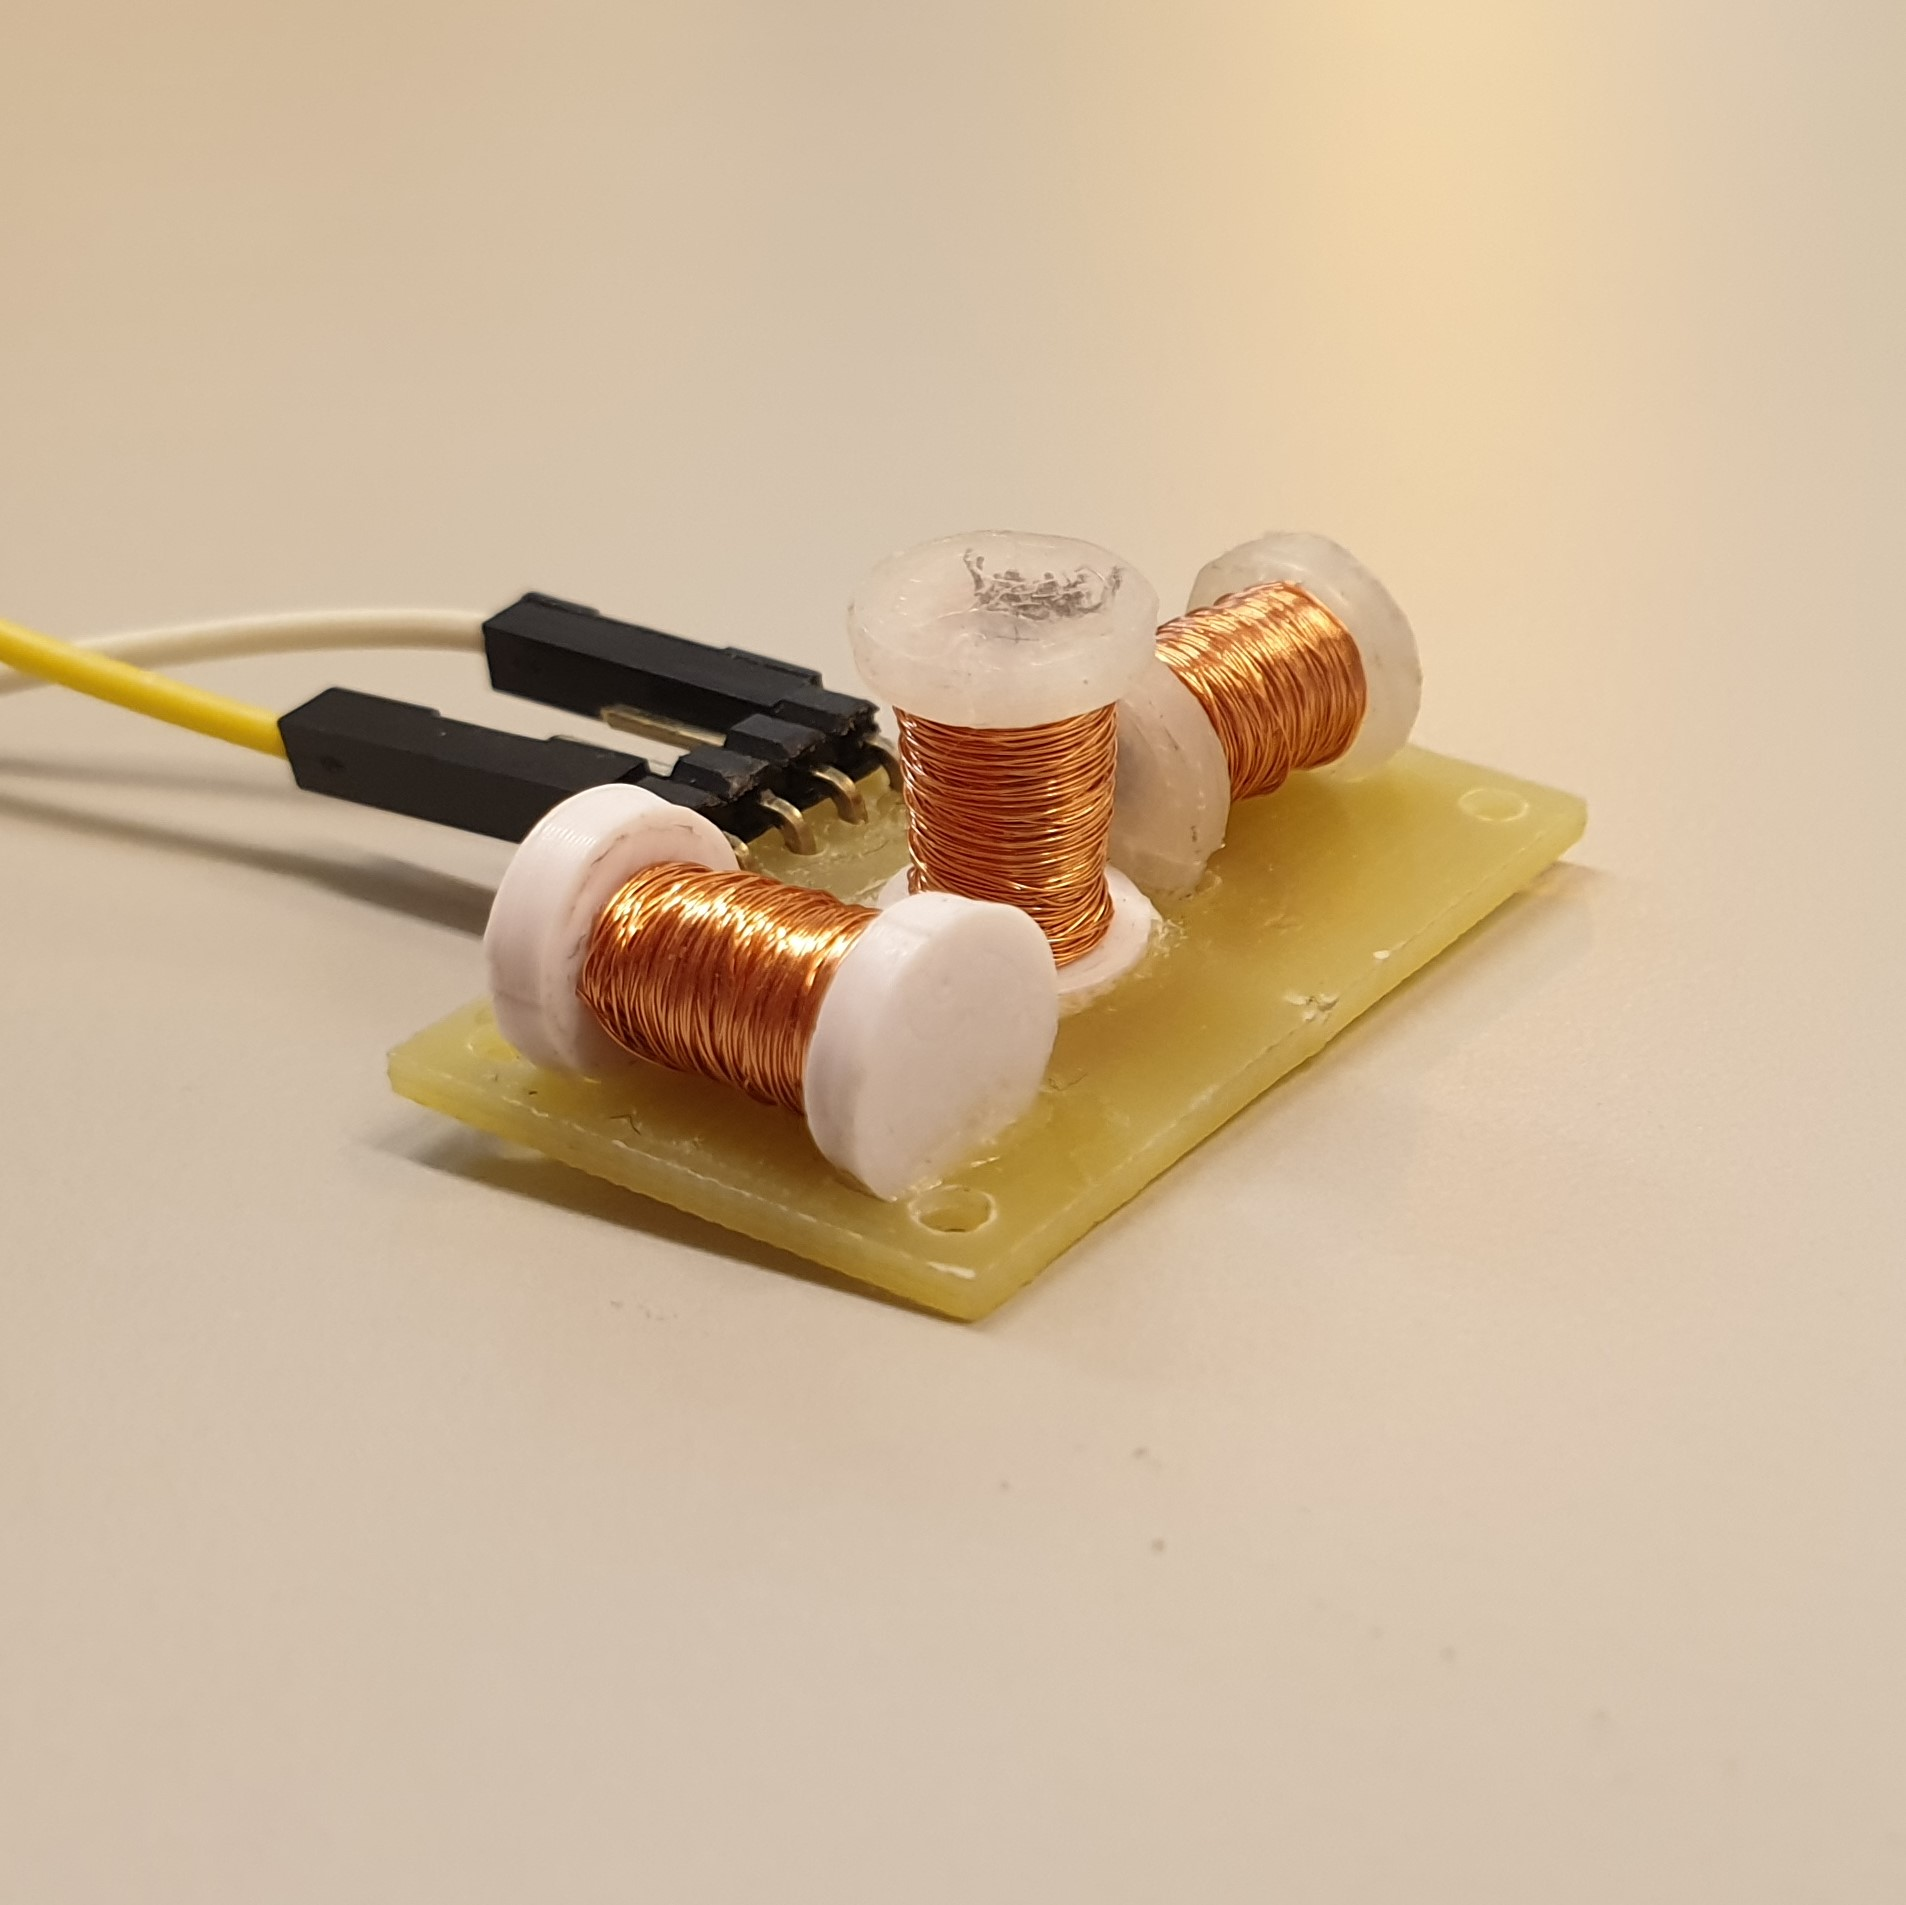
\includegraphics[width=\textwidth]{images/Spolhubb1.jpg}
    \vfill

    \begin{large}
        Lärosäte: ABB-Gymnasiet\\
        \vspace{0.5cm}
        Klass: 190S\\
        \vspace{0.5cm}
        Handledare: Andreas Jillram, ABB-Gymnasiet
    \end{large}

\end{titlepage}


\begin{abstract}

\end{abstract}

\begin{otherlanguage}{english}
    \begin{abstract}
    \end{abstract}
\end{otherlanguage}

\tableofcontents

\newpage
\pagenumbering{arabic}

\begin{sloppypar}

    \section{Inledning}
    \subsection{Syfte}
    Syftet med projektet är att undersöka hur människan finmotoriska rörelser kan detekteras, hur rörelserna såsom fingerrörelse kan användas som inmatning till olika system
    och utveckla ett prototyp som kan både detektera och återskapa fingerrörelser från en människohand.
    De finmotoriska rörelser kan återskapas antingen med en digital representation av rörelsen eller med en fysisk robothand.
    % De detekterade rörelserna ska sedan översättas till data som går att visualisera exempelvis genom att kontrollera en fysisk robothand eller digitalt i ett datorprogram.
    \subsection{Bakgrund}
    Det finns ett ökat intresse och en ökad efterfrågan på olika sätt för människan att interagera med datorer och robotar.
    Bland annat hur människokroppen kan användas för inmatning till datorprogram och till olika maskiner.
    Den här tekniken är som mest utvecklad inom virtual reality och augmented reality och det är inom dessa områden som tekniken i nuläget har störst användning.
    Tekniken är dock fortfarande relativt begränsad och använder mestadels grövre motorik som inmatning och förlorar den precision som kan ges av finmotoriska rörelser.

    % Vi ser ett ökande intresse för andra applikationer där människan agerar fjärrkontroll.   

    \subsection{Frågeställning}

    \section{Teori}
    För att få en bättre bild av hur en robothand kan skapas och styras med hjälp av olika sensorer undersöktes andra, liknande projekt.
    Projektet drog inspiration från en kandidatexamen från två KTH-studenter~\cite{KTHhand} med ett liknande syfte, och
    idéer för tummens funktion på den fysiska handen kom från ett projekt som hette \textit{Etho Hand}~\cite{EthoHand}
    vars syfte var att utveckla en hand som kunde utföra komplexa rörelser.


    \subsection{Elektromagnetism}
    \subsubsection{Magnetfält}
    Magnetfält är fält som rör sig i en riktning från nord- till sydpolen på en magnet eller runt en strömförande elektrisk ledare.
    Den magnetiska flödestätheten, ekvivalent med magnetfältets \textit{styrka}, kring en ledare med ström, avtar med avstånd från ledaren,
    vilket är relevant för detta projekt.~\cite{digilar}
    \subsubsection{Induktion}
    Inducerad spänning är spänning som alstras när en ledare befinner sig i ett magnetfält, på grund av att de laddade partiklarna hamnar på motsatta sidor av ledaren.
    Det skapar en skillnad i laddning, vilket korrelerar med spänning.
    Enligt Lenz lag ger denna spänning upphov till en ström, i en sluten krets, och att strömmens riktning motverkar förändringen av det magnetiska flödet.
    Denna princip kan användas för att alstra ström ur ett magnetfält, exempelvis i en generator.
    Induktion fungerar också åt motsatt håll: ström och spänning i en krets ger upphov till magnetfält runt ledaren.
    ~\cite{digilar}

    \subsection{Elektronik}
    \subsubsection{Spolar}
    En spole är en ledare som lindats i varv på ett sådant sätt att magnetfältet som skapas när ström flödar igenom har en nord- och en sydpol.
    Spolar kan lindas runt ett material, en \textit{kärna} som förstärker magnetfältet, eller bara med luft i mitten.
    På grund av att spolen inducerar spänning kommer den motverka strömmen i kretsen den ingår, enligt Lenz lag, vilket bland annat ger en förskjutning mellan spänning och ström, i en växelströmskrets.~\cite{digilar}
    \subsubsection{Mätning av spolar}
    För att dimensionera en krets kan det vara viktigt att veta vilka värden ens komponenter har.
    Till restistorer och kondensatorer är detta oftast enkelt, då de flesta moderna multimetrarna kan mäta resistans och kapacitans.
    Verktyg för att mäta spolars induktans (som mäts i enheten 1 Henry) är sällsyntare, och därför finns olika metoder för att själv mäta spolar utan specialverktyg.
    För detta kan exempelvis en funktionsgenerator och ett oscilloskop användas, och genom att utnyttja spolens upp- och urladdningsförmåga kan man approximera spolens induktans.
    En sinusformad spänning med amplituden 0,5~V utan något annat inkopplat kommer minska när en spole kopplas parallellt med mätverktyget. Genom att ändra frekvensen kan man uppnå signalen med 0,5~V amplitud.
     Denna frekvens $f$ tillsammans med resistansen $R$, som mäts med multimeter när ingen spänning ligger över den, kan användas för att räkna ut induktansen $L$ enligt formel \ref{eq-inductance}.~\cite{MeasureInductor}

    \begin{equation}
        \label{eq-inductance}
        L = \frac{\sqrt{\frac{2500+100R-3R^2}{3(2\pi)^2}}}{f}
    \end{equation}


    \subsubsection{Kondensatorer}
    Kondensatorn är en elektrisk komponent som kan lagra elektrisk energi, genom att laddas upp och laddas ur med spänning, vilket ger upphov till en förskjutning mellan ström och spänning, i en växelströmskrets.~\cite{digilar}

    \subsubsection{Operationsförstärkare}
    En operationsförstärkare är en förstärkare som förstärker spänningsskillnaden mellan operationsförstärkarens ingångar enligt formel \ref{eq-Op-Amp} där $A_{OL}$ är amplifikationen i en öppen loop.~\cite{wiki:Operational-amplifier}
    \begin{equation}
        \label{eq-Op-Amp}
        V_{out} = A_{OL}(V_+ - V_-)
    \end{equation}
    

    \subsubsection{Filter}
    Ett elektroniskt filter är en elektrisk komponent som används för att filtrera bort oönskade frekvenser från signaler. ~\cite{wiki:Electronic-filter} 
    En typ av elektroniskt filter är aktiva filter, där aktiva komponenter används såsom operationsförstärkare används för att förbättra prestanda och förutsägbarhet för filtret samt för att sänka priset. 
    Operationsförstärkaren förhindrar också följande krets belastning från att påverka filtrets egenskaper. ~\cite{wiki:Active-filter}
    För att filtrera alla signaler förutom signaler med en frekvens inom ett visst intervall kan ett band-pass filter användas. ~\cite{wiki:Band-pass-filter}

    \subsubsection{Oscillatorer}
    En oscillator är en elektrisk krets eller en del av en elektrisk krets där växelström, ström som regelbundet byter riktning, skapas.
    På grund av spolars och kondensatorers upp- och urladdningsförmåga kan dessa användas, i olika kombinationer för att göra en krets där strömmen och spänningen svänger (blir svagare/starkare, och byter riktning) med en viss frekvens.
    Oscillatorer är användbara om man vill skapa växelström med en likströmskälla, vilket för det här projektet är mycket relevant för att kunna alstra ett varierande magnetfält i spolarna.

    En sorts oscillator är en Wien-bryggeoscillator (\textit{Wien Bridge Oscillator})~\cite{WienBridge} där resistorer, kondensatorer och en operationsförstärkare används för att skapa en vågformad växelströmssignal, där frekvensen bestäms av resistorernas och kondensatorernas värden.
    En annan sorts oscillator är en 555-oscillator~\cite{555_sine}, som bygger på ett chip med en integrerad krets (\textit{IC}) vid namn 555. 555-chippet kan ge fyrkantsformade utsignaler om de sätts i ett visst värde, och där frekvensen bestäms med hjälp av restistorer och kondensatorer. Det går också att filtrera signalen så att den liknar en sinusvåg, med hjälp av en spole och kondensatorer.

    \subsubsection{Arduino Nano 33 BLE}
    Arduino Nano 33 BLE är en mikrokontroller baserad på kretsen Nordic nRF52480 producerad av företaget Arduino.
    Arduino Nano 33 BLE är en fysiskt liten mikrokontroller. Nordic nRF52480 är bestyckad med en Cortex M4F processor
    och en NINA B306 BLE-modul som möjliggör kommunikation med Bluetooth Low Energy. Arduino Nano 33 BLE har 8 analoga
    ingångar och kan drivas av spänning mellan 4,5 och 21 volt. Annan viktig hårdvaruinformation om mikrokontrollern
    kan ses i tabell~\ref{table:ArduinoNano}. ~\cite{Arduino:ABX00030}\\\
    Mikrokontrollern används för att läsa av mätvärden från sensorerna och för att skicka vidare mätvärdena till
    datorn där renderingen sker. Den programmeras i C++ med hjälp av platformIO, en tillbyggnad i utvecklingsmiljön
    Visual Studio Code som möjliggör programmering av mikrokontrollers i C++.

    \begin{table}[h]
        \begin{center}
            \caption{Viktiga specifikationer Arduino Nano 33 BLE ~\cite{Arduino:ABX00030}}
            \label{table:ArduinoNano}
            \begin{tabular}{ | l | l | }
                \hline
                Mikrokontroller            & nRF52840 \\
                \hline
                Driftspänning              & 3,3V     \\
                \hline
                Inspänning (min)           & 4,5V     \\
                \hline
                Inspänning (max)           & 21V      \\
                \hline
                Digitala ingångar/utgångar & 14 st    \\
                \hline
                Analoga ingångar           & 8 st     \\
                \hline
                Längd                      & 45 mm    \\
                \hline
                Bredd                      & 18 mm    \\
                \hline
            \end{tabular}
        \end{center}
    \end{table}
    \subsection{Bluetooth Low Energy}
    Bluetooth Low Energy liknar traditionell Bluetooth, men är mer energieffektiv.
    \subsubsection{Peripheral}
    \subsubsection{Central}

    \subsection{Rendering}
    \subsubsection{Unity}
    Unity är en programvara som möjliggör skapandet av real-time 3d-miljöer för spel, film etc. https://unity.com/our-company.

    \subsection{Tidigare lösningar}
    För att få bättre uppfattning av hur industrin för fingerspårning ser ut idag beskrivs här de metoder som undersöktes under projektets planering.
    \subsubsection{Computer vision}

    \subsubsection{Inertial measurement unit (IMU)}
    Inertial measurement unit är en slags sensor som mäter av rörelser. Genom att
    placera sensorer på de olika fingersegmenten på handen kan rörelser i tre
    dimensioner spåras. Precis spårning kräver minst 16 sensorer placerade på
    handen. Det finns även lösningar med IMU-sensorer som använder 7 sensorer
    där där övriga positioner antas utifrån de positioner som läses in.\cite{wiki:Finger_tracking}

    \subsubsection{Flexsensor}
    En flexsensor är en sensor som ändrar resistans proportionerligt med hur mycket den är böjd \cite{wiki:Flex_sensor}.
    Flexsensorer kan användas för att mäta hur mycket ett finger är böjt och de har använts i projekt och produkter för att spåra böjning, till exempel genom att integrera flexsenorer i en handske för att styra olika applikationer. Ett exempel är datahandsken \cite{wiki:Wired_glove}, som används bland annat för att känna igen teckenspråk.

    \subsubsection{Magnetfält}
    Att mäta avtånd och rotation av fingrar och händer är något ovanligare inom industrin, men många exempel kan hittas som examensprojekt på olika högskolor i flera länder.
    Många av dessa projekt liknar detta gymnasiearbete, med liknande syfte och grundläggande metod, men med lite annorlunda tillvägagångssätt.
    Ett projekt använder sig av maskininlärning för att bättre kunna förutspå fingerposition~\cite{article:sci-rep-mag-ind}.
    Projektet \textit{AuraRing}~\cite{article:AuraRing} använder sig av en ring runt fingret som skickar ut magnetfält, som sedan kan plockas upp av fem spolar på handleden för att få en bättre bild av fingrets position.
    De använder sig av både maskininlärning och en mer traditionell iterativ metod för att uppnå sin mätning.
    Ett annat projekt, \textit{MagIK}~\cite{article:MagIK}, använder spolar på fingrarna samt en rad spolar på handryggen för att kunna räkna ut position utan AI, men använder sig av kamera för att verifiera den uppmätta positionen.
    Detta är alltså något som inte är vanligt inom industrin, och en metod som kan tillämpas och utforskas på olika sätt.

    \section{Metod och material}


    Projektet började med att undersöka hur spårning av handrörelser har gjorts tidigare. 
    Där följde undersökningar i hur en människohand fungerar och hur en fysisk hand kan konstrueras. 
    Projektet delades sedan in i två processer, en process för att skapa ett sensorsystem som kunde användas för att spåra fingerrörelser, 
    och en annan process för att skapa en representation av den data som mäts in av sensorsystemet, som arbetades på parallellt.

    \subsection{Process 1 - Sensor}

    \subsubsection{Material}

    \subsubsection{Val av metod}
    Metoden som valdes var att spåra fingrarna med hjälp av spolar på finertopparna som
    sänder ut ett magnetfält som genom att läsas av skulle kunna ge finrarnas rotation
    och position. Valet av metod stod mellan tre huvudkandidater. Avläsning av magnetfält
    från spolar på fingertopparna, flexsensorer för att ta fram fingrarnas rotation, eller
    flertalet IMU-sensorer som genom att mäta röreslerna på olika delar av handen kan
    ge data på hur hela handen rör på sig.
    Metoden med accelerometrar valdes bort tidigt eftersom det var en väldigt avancerad och
    dyr metod som skulle kräva minst 7 stycken sensorer för att fungera och minst 16 stycken
    sensorer för att kunna spåra hela handen. Då metoden krävde mycket för att komma
    igång bedömdes den icke-länplig för projektet.
    Metoden med flexsenorer var den metod som bedömdes som lättast att genomföra. Metoden
    valdes bort på grund av att flexsensorer ansågs för begränsande då flexsensorerna
    endast fanns i specifika storlekar som gjorde att vissa positioner och rotationer
    skulle vara svåra att mäta. Flex-sensorerna som sensorer var även väldigt dyra och
    metoden bedömdes vara aningen enkel och hade redan gjorts många gånger tidigare.
    Dessutom kan en flexsensor endast mäta rörelse i en riktning vilket innebar att
    precis mätning av alla fingrars rörelser skulle kräva ett stort antal sensorer.
    Slutligen valdes magnetfält eftersom det verkade som en lovande metod. Magnetfält
    används till största delen för att spåra grövre rörelser men bedömdes ha potential
    att mäta även finare röresler. Metoden var även den som var minst beprövad vilket
    innebar att gruppen skulle behöva ägna sig åt mera testning och utforkning.


   

    \subsubsection{Spolar}
    Spolar användes för att skapa och läsa av magnetfältet som används för att läsa av fingrets position och rotation.
    En spole består av en järnkärna, 0,1 mm koppartråd samt 3D-printade hattar
    För att få lämplig storlek och funktion från spolarna valdes ett varvtal på 1000 varv.
    Spolarna konstruerades genom att limma fast hattar i ändarna på järnkärnan.
    Sedan lindades spolarna med koppartråd.
    Lindningen gjordes genom att fästa den olindade spolen i en motor som genom att snurra samtidigt som koppartråd
    var fäst i den olindade spolen gjorde att järnkärnan lindades med koppartråden.
    Motorn var kopplad till en Arduino mikrokontroller som med hjälp av en varvmätare kunde läsa av hur många varv
    koppartråd som hade lindats runt spolen.
    När mikrokontrollern räknat att motorn roterat 1000 varv stängdes motorn automatiskt av. Se figur \ref{fig:Spolsnurrare}.
    Kod för spolsnurraren finns i bilaga \ref{bilaga:Kod_Spolsnurrare}

    \begin{figure}[H]
        \centering
        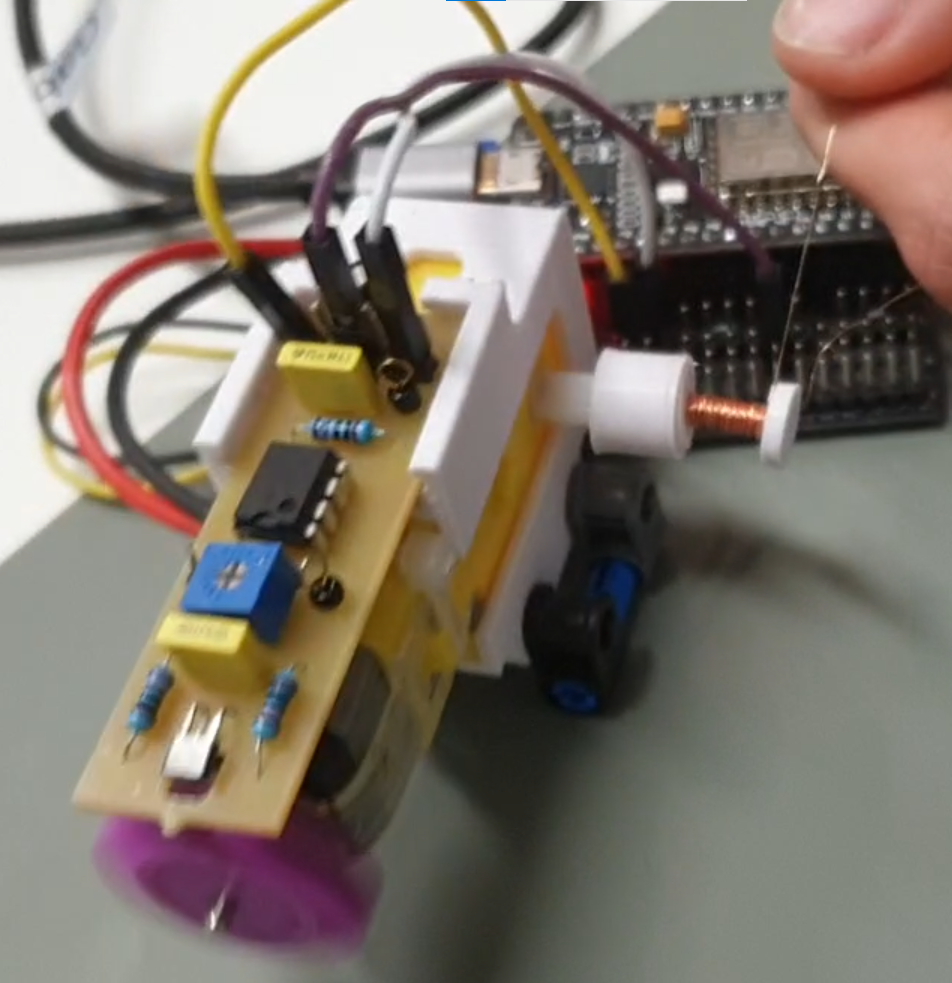
\includegraphics[width=0.6\textwidth]{spolsnurrare1.png}
        \caption{Bild från när en spole lindades med hjälp av Spolsnurraren.}
        \label{fig:Spolsnurrare}
    \end{figure}

    De färdiga spolarna mättes sedan med oscilloskop och funktionsgenerator för att säkerställa dess induktans, för att användas i oscillatorkretsen.
    Den första spolen som färdigställdes jämfördes också med spolar som anväds i utbildningssyfte inom fysik, för att säkerställa att de hade samma funktion.
    Detta genom att använda två fysik-spolar för att skicka och ta emot signaler, där en spole var kopplad i serie med en funktionsgenerator som genererade en sinusformad signal, och där den andra var kopplad till ett oscilloskop för att läsas av.
    En av fysik-spolarna byttes sedan ut mot den egensnurrade spolen, för att se om signalen kunde skickas och tas emot av dessa.

    För att få bättre kontakt med andra kablar och komponenter valdes ett antal spolar ut för att lödas fast i kablar av större tjocklek.
    Jämförelsen mellan en spole med fastlödd kabel och en spole utan fastlödd kabel kan ses i figur \ref{fig:SpoleVsSpole}.

    \begin{figure}[H]
        \centering
        \includegraphics[width = 0.6\textwidth]{spole-vs-spole.jpg}
        \caption{En spole med endast hatt, kärna och lindning (överst) och en spole med kablar fastlödda (underst).}
        \label{fig:SpoleVsSpole}
    \end{figure}


    \subsubsection{Montering på hand} %3d prints,  etc. bättre titel
    För att montera spolar på handen monterades de tre mottagarspolarna på ett kretskort som agerade spolhubb.
    De tre spolarna monterades i varsin riktning så att de kan ta upp fingerrörelser i tre dimensioner.
    Kretskortet modellerades i ultiboard och frästes sedan ut på skolan kretskortsfräs.
    På kretskortet monterades spolarna genom att limmas fast i kretskorten och koppartråden löddes fast på kortets undersida.
    För att kunna skicka vidare signalen som spolarna plockar upp löddes även en stiftlist fast på kretskortet.


    \subsubsection{Filter}
    Filtret ska filtrera frekvenser som inte är inom ett visst frekvensområde och ett aktivt bandpassfilter valdes som filtertyp.
    Filterkretsen designades först med hjälp av formler för att bestämma värden på kondensatorer och resistorer.
    Kretsen testades sedan i simulering för att säkerställa att kretsens fungerar som förväntat,
    dock användes en ideal operationsförstärkare under simuleringen.
    När kretsen sedan simulerades med icke-ideal operationsförstärkare kunde kretsen inte längre filtrera signalen.
    Det visades sig att formlerna för kondensatorer och resistorer
    antog att operationsförstärkare var ideal för att kretsen skulle fungera.
    Kretsen designades sedan om med hjälp av ett filter designverktyg av Texas Instruments
    och fungerade i simulering med en icke-ideal operationsförstärkare.

    \subsubsection{Oscillator}
    För de olika fingrarna bestämdes att oscillatorerna skulle ha frekvenser från 100 kHz, med ungefär 15 kHz mellanrum för att ge utrymme för filtrernas bandbredd. Fem oscillatorer behövdes, ett för varje finger.
    Ursprungligen planerades att använda oscillatorer som bygger på wienbryggor (Wien-bryggesoscillator).
    Till detta skulle behövas resitorer, kondensatorer och operationsförstärkare. Resistorer och kondensatorer dimensionerades och kretsen simulerades i program för att kontrollera att allt stämde.
    Efter förslag om att integrera spolarna i kretsen som en resonanskälla byttes oscillatorerna mot 555-oscillatorer.
    Här dimensionerades istället två olika kretsar i en: en med resistorer och kondensatorer, och en med kondensatorer och spolen.

    Två oscillatorer byggdes i verkligheten: en med frekvensen 100 kHz och en med frekvensen 117 kHz.
    I 117 kilohertz-kretsen användes ett 556-chip, som har samma funktioner som två stycken 555:or; en på varje sida av komponenten, och som drar mindre effekt. Se bilaga för kretsschema.

    
    \subsection{Process 2 - Representation}

    \subsubsection{Material}
    
    \subsubsection{3D-hand}
    En 3D-printad fysisk hand designades som skulle imitera den rörelse som spårats med sensorsystemet.
    Designen bestod av fingersegment som kunde skrivas ut med en 3D-skrivare och 7 servon som med hjälp av trådar skulle böja fingrarna.

    \subsubsection{Mikrokontroller}
    Mikrokontrollen Arduino Nano 33 BLE används för att kommunicera med renderingsprogrammet.
    Mikrokontrollen väntar på renderingsprogrammet att ansluta och
    läser sedan av värdena från de olika sensorerna och publicerar dessa till en Bluetooth characteristics.
    För att åstadkomma kommunikation används biblioteket ArduinoBLE.

    \subsubsection{Renderingsprogram}
    Ursprungligen skulle ett CSharp program skapas som kunde kommunicera med mikrokontrollen som sedan också skulle renderar fingerrörelserna.
    Istället för att skapa ett eget renderingsprogram beslutades det att spelmotorn Unity skulle användas.
    Kommunikationen mellan mikrokontrollen och renderingsprogrammet sköttes därav istället av biblioteket BleWinrtDll som är går att direkt integrera med Unity
    och en färdig konstruerad modell från Ultraleaps Unity Plugin användes för att representera fingerrörelse.
    Unity programmet skulle anslutas till mikrokontrollen som sedan skulle översätta värdena från sensorerna till rotationer i fingrarnas leder.
    Programmet testades genom att skicka två specifika värden från mikrokontrollen till Unity-programmet som roterade ett fingers leder till två olika rotationer beroende på vilket värde som skickats.

    \section{Resultat}

    \subsection{Oscillator}
    \subsubsection{Spolar}
    De egentillverkade spolarna hade samma funktion som andra fabrikstillverkade spolar, enligt den jämförelse som gjordes.
    Signalen var något förändrad vad gäller amplitud, men hela signalen kunde tas emot.
    Störningar från omgivningen var dock något större, enligt resultaten som kunde ses i oscilloskop.\\\\
    Första mätningen av de första tre spolarnas induktans gav en genomsnittlig induktans på 3,3 mH vilket användes vid dimensionering av oscillatorer.
    Vid en andra omgång mätningar mättes fem andra spolar, där den genomsnittliga induktansen var runt 7,0 mH, vilket ledde till att oscillatorkretsarna dimensionerades om. Se tabell \ref{table:inductance}

    \begin{table}[H]
        \begin{center}
            \caption{Uppmätta induktanser i egensnurrade spolar. Värdena från första mätningarna är runt 3,3~mH och de från andra mätningen är runt 7,0~mH.}
            \label{table:inductance}
            \begin{tabular}{| l | l |}
                \hline
                Spolnummer & Induktans (mH) \\
                \hline
                1          & 3,3            \\
                2          & 3,3            \\
                3          & 3,53           \\
                4          & 6,86           \\
                5          & 7,03           \\
                6          & 7,12           \\
                7          & 7,03           \\
                8          & 7,23           \\
                \hline
            \end{tabular}
        \end{center}
    \end{table}
    Under testning gick vissa spolar sönder, och lödningen släppte på två av fyra lödda spolar under laborationer och tester.

    \subsubsection{Oscillatorkrets}
    I simuleringar gav oscillatorkretsarna signaler med amplituder (maxvärden) från 3~V till 5~V. Se figur \ref{fig:sim-117kHz}.

    \begin{figure}[H]
        \centering
        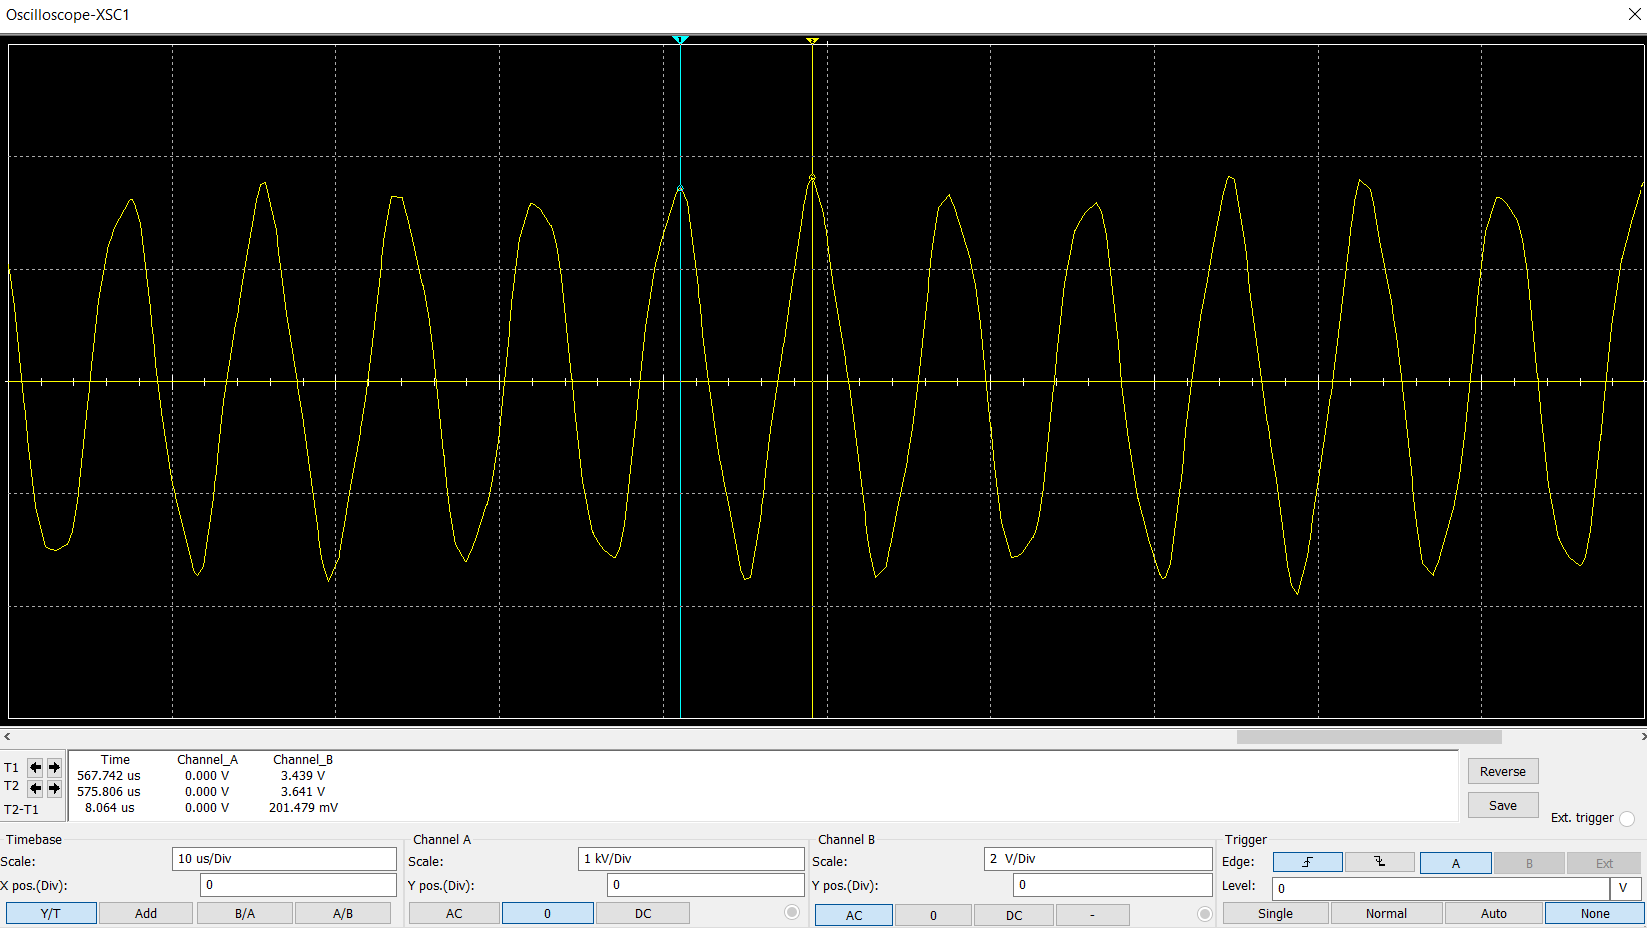
\includegraphics[width=\textwidth]{multisim-signal-555-117kHz.png}
        \caption{Bild av simulerad oscillator med dimensionerad frekvens 117 kHz, tagen i Multisim.}
        \label{fig:sim-117kHz}
    \end{figure}

    Kretsen som dimensionerades för 100~kHz, som använde ett 555-chip, gav signaler som endast skiljde sig från omgivningens störningar med någon millivolt, och vars frekvens rimligtvis kunde antas vara ungefär 10 gånger större än 100 kilohertz.
    Då spolen som ingick i kretsen gick sönder kunde fler tester inte utföras.

    Kretsen som skulle ge 117~kHz, med 556-chippet, gav en signal med amplitud på cirka 5,5~mV, och frekvens som varierade mellan 115~kHz och 130~kHz.
    Signalen var inte helt sinusformad men oscillerade mellan positiv och negativ spänning i sågtandsliknande vågor. Se figur \ref{fig:signal-117kHz}.

    De komponenter som användes hade inte exakta värden enligt mätningar som gjordes vid kopplingen. Resistorerna hade felmarginaler mellan 1 och 5\%, medan kondensatorerna hade felmarginaler från 10 till 30\%.

    \begin{figure}[H]
        \centering
        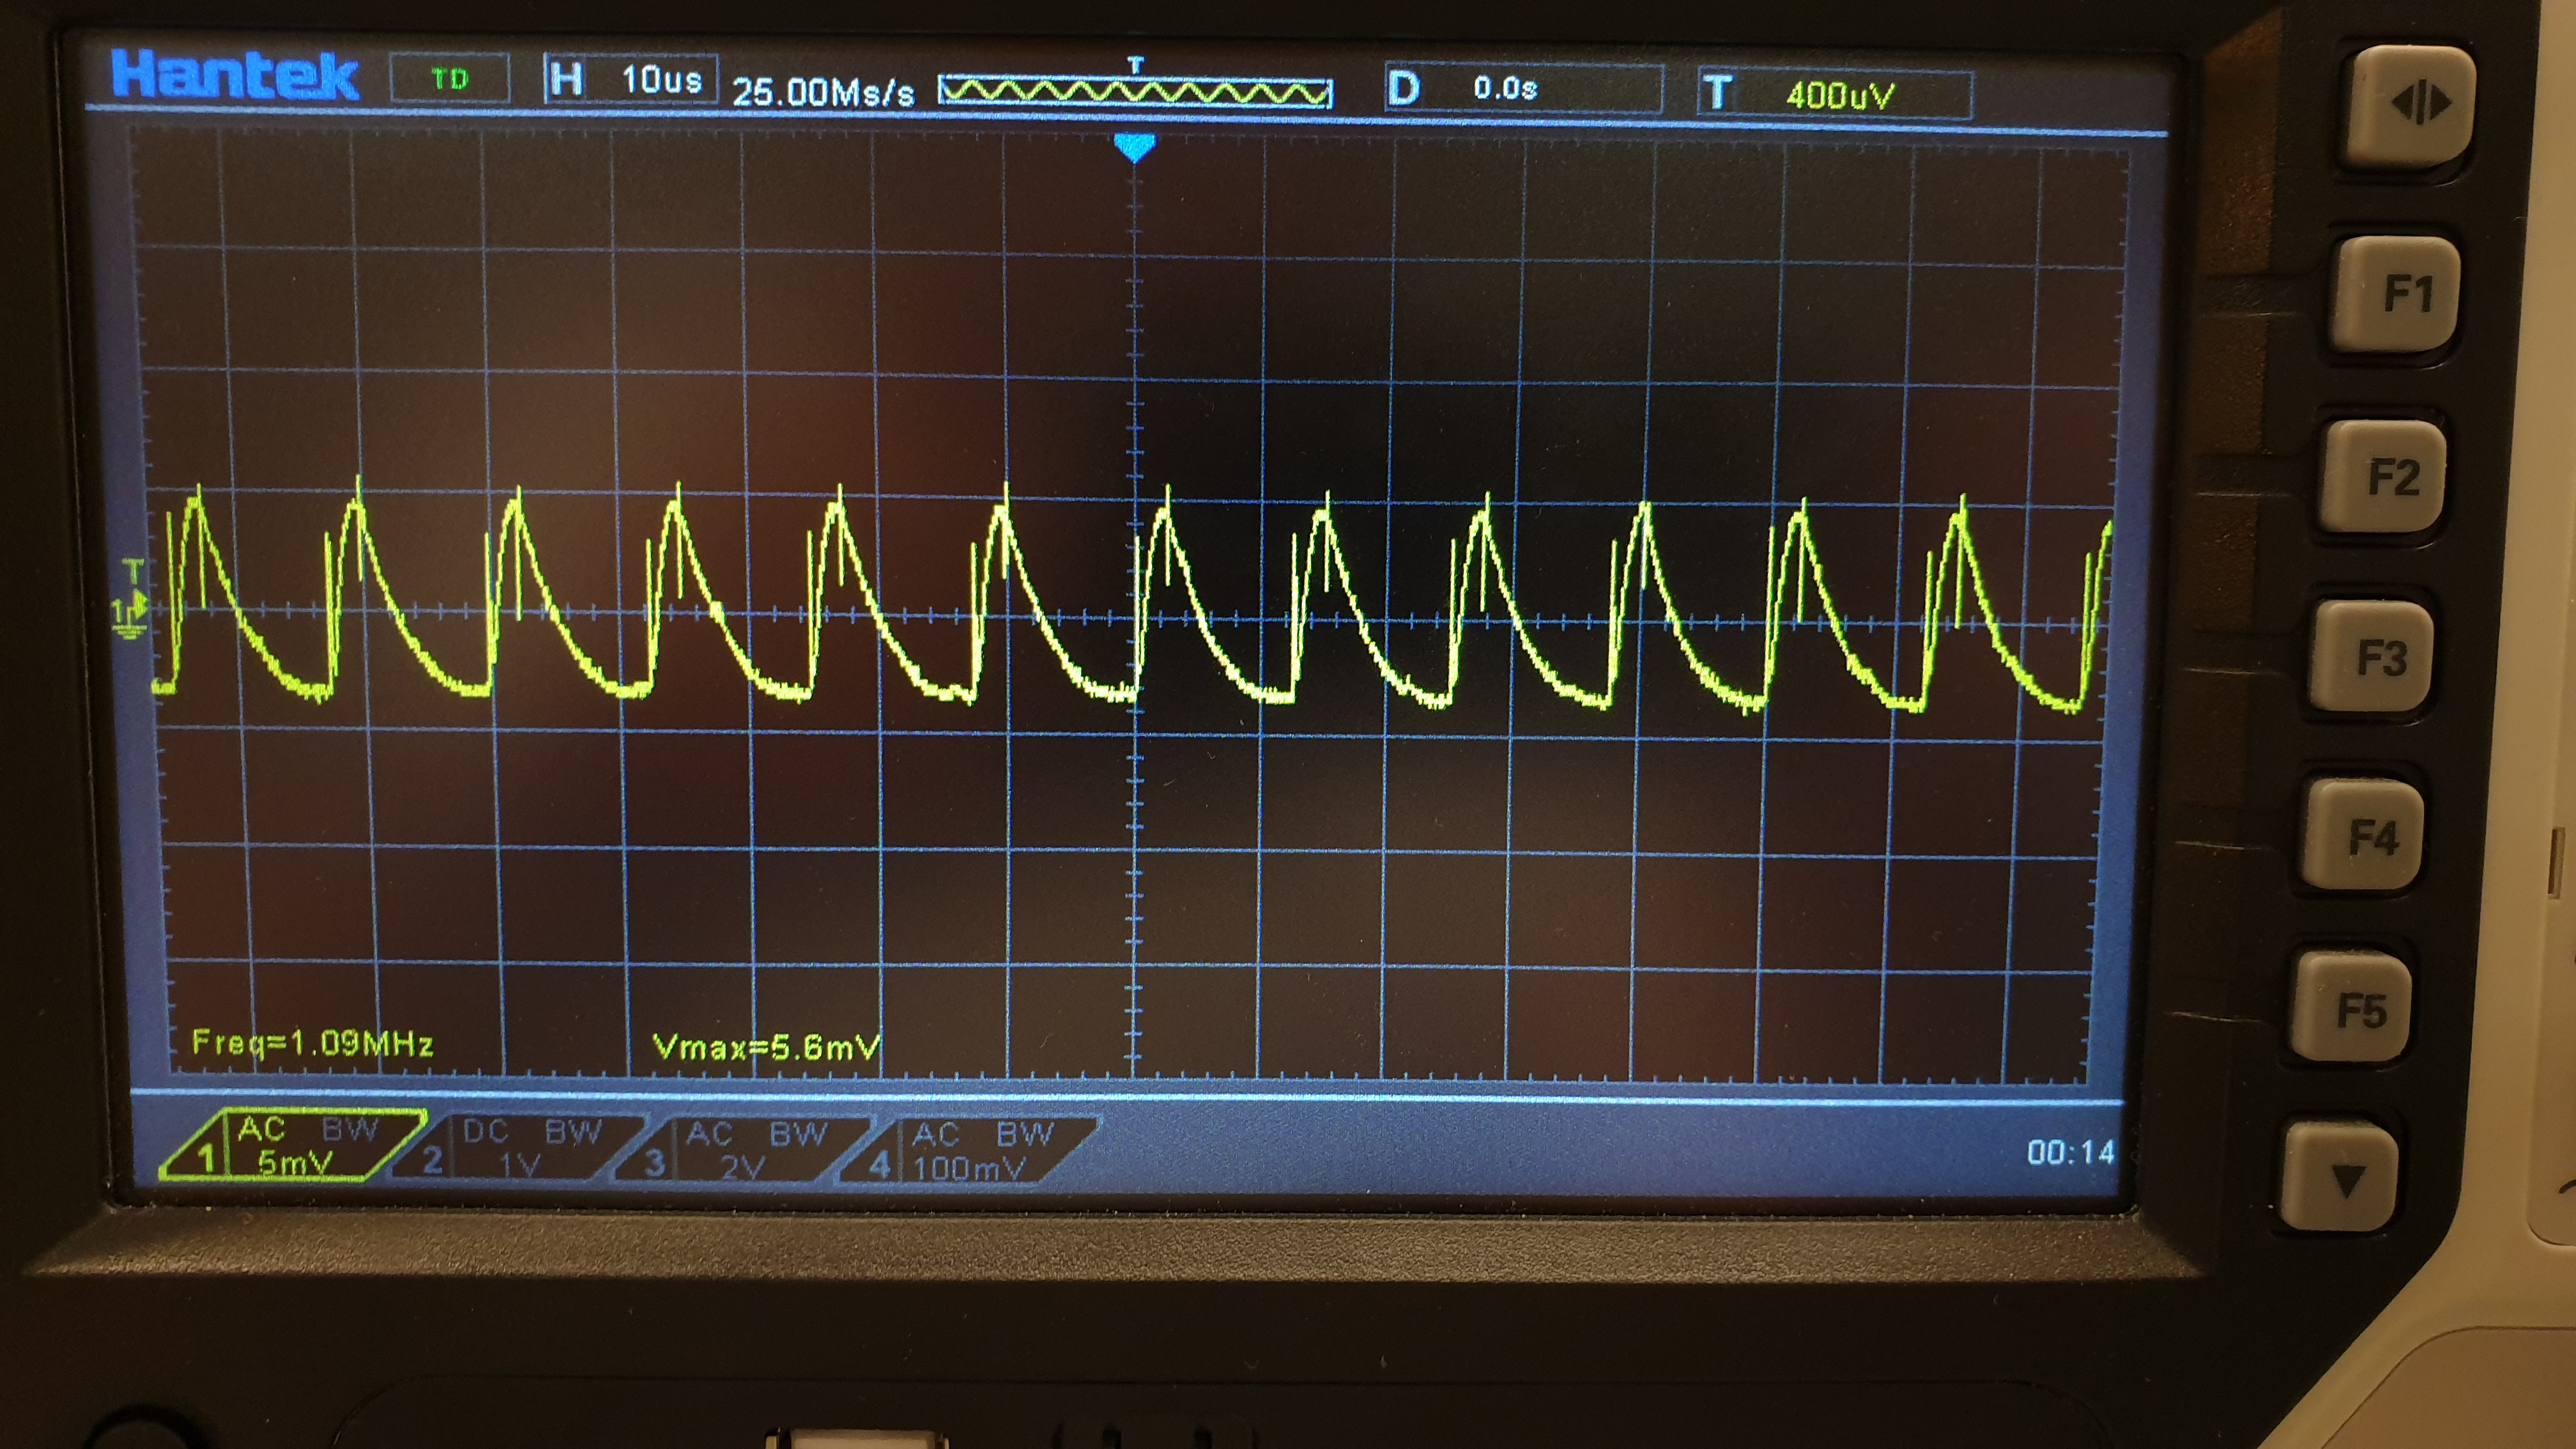
\includegraphics[width = 0.9\textwidth]{signal-555-117kHz.jpg}
        \caption{Oscillatorbild av signal från 117~kHz-oscillatorkretsen. Nere till vänster kan man se spänningens maxvärde, och hur stor frekvens signalen har (med störningar).}
        \label{fig:signal-117kHz}
    \end{figure}

    \section{Diskussion och Slutsats}
    %\subsection{Diskussion}
    \subsection{Spårning}
    \subsubsection{Oscillator}
    % Lägg till mer
    Oscillatorerna fungerade inte som planerat, och gav andra resultat än de som hade simulerats.
    100~kHz-oscillatorns svaga och knappt urskiljbara signaler var svåra att tolka, då de påminde om kondensatorers upp- och urladdnigscykler när systemet var av (ingen matningsspänning) och blev mer fyrkantsformade när kretsen hade matningsspänning.
    Den svaga signalen antogs kunna filtrerats och sedan förstärkts, när filterkretsen väl hade blivit byggd.
    Felet kan ha berott på många faktorer, exempelvis att komponenterna var tvungna att ha mer exakta värden.
    I simuleringar behövde kondensatorerna vara väldigt exakta för att spänningen i kretsen skulle ge upphov till resonans och bli starkare.
    Att kondesatorerna hade så stora felmarginaler kan ha gjort att kretsen inte fungerade som den skulle, men enligt nya simuleringar bör det inte ha påverkat resultatet så mycket.

    En annan felkälla kan vara att spolarnas induktans mättes felaktigt. Resultaten från mätningarna har ännu inte verifierats med andra verktyg eller metoder, vilket innebär att mätningarna kan vara felaktiga.
    Detta upptäckte vi redan vid den andra gångens mätningar, där induktansen drastiskt ändrades från 3,3~mH till 7~mH, trots att spolarna var mycket lika i varvtal, material och storlek. Om den första mätningen var fel finns en större risk att andra mätningen också är fel, och det skulle innebära att kretsens andra komponenter var feldimensionerade.

    Ännu en potentiell felkälla som kan förklara signalens låga maxvärden jämfört med simuleringarna kan vara att respektive 555 och 556 ger för svaga spänningar. Enligt databladen, de guider som följdes och simuleringarna som gjordes skulle 555:an ha en utspänning runt 4 till 5~V, medan den här låg på bara några millivolt.
    Vad detta beror på är för tillfället okänt, men det är tydligt att 555:an och 556:an har haft stor inverkan på projektets resultat, och speciellt oscillatordelens resultat.
    \subsubsection{Filter}

    \subsection{Visualisering}
    \subsubsection{3D-utskriven hand}
    \subsubsection{Digital hand}

    \subsection{Planering}

    \subsection{Slutsats}

    \section{Avslutning}




    \section{Källor}
    \printbibliography[heading=none]

    \appendices
    \titleformat{\section}[display]
    {\normalfont\Large\bfseries}{\appendixname\enspace\thesection}{.5em}{} %ny rad efter bilaga x
    \section{Renderingskod}

    \section{Oscillatorkretsar}
    Kretsar för 100 kHz (överst) respektive 117 kHz (underst). Kretsarna är gjorda i Multisim.

    \label{bilaga:Schema-Oscillatorkretsar}
    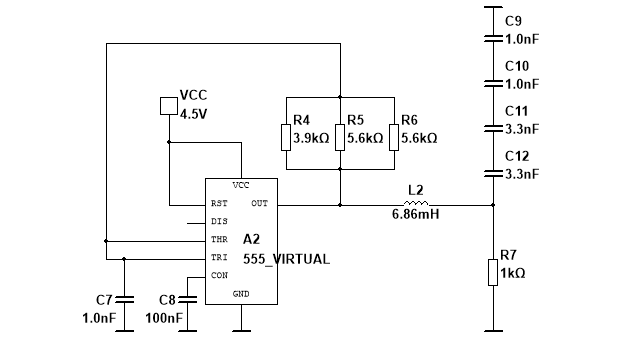
\includegraphics[width = 0.8\textwidth]{555-100kHz-circuit.png}
    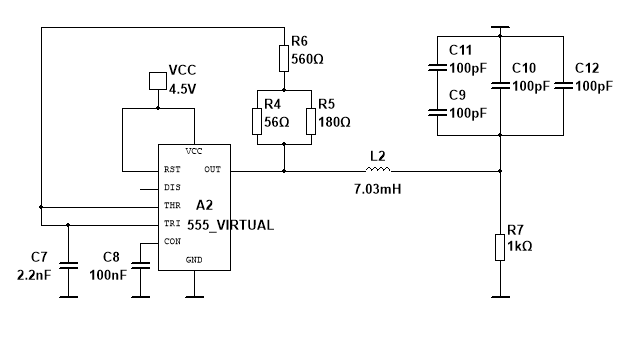
\includegraphics[width = 0.8\textwidth]{555-117kHz-circuit.png}




    \section{Filterkrets}

    \inputminted[breaklines]{cpp}{./Code/Spolsnurrare.cpp}

    \section{Kod Arduino Peripheral}
    \label{bilaga:Kod_Arduino_Peripheral}
    \inputminted[breaklines]{cpp}{./Code/peripheral.cpp}

    \section{Kod Rendering}
    \label{bilaga:Kod_Rendering}
    \inputminted[breaklines]{csharp}{./Code/handController.cs}
    \newpage
\end{sloppypar}


\end{document}